\documentclass{article}
\usepackage{amsmath}
\usepackage{hyperref}
\usepackage{tikz}
\usetikzlibrary{calc,arrows,shapes,positioning}
\usepackage{float}
\usepackage{xstring}
\usepackage{catchfile}

\CatchFileDef{\headfull}{../.git/HEAD}{}
\StrGobbleRight{\headfull}{1}[\head]
\StrBehind[2]{\head}{/}[\branch]
\IfFileExists{../.git/refs/heads/\branch}{%
    \CatchFileDef{\commit}{../.git/refs/heads/\branch}{}}{%
    \newcommand{\commit}{\dots~(in \emph{packed-refs})}}
\newcommand{\gitrevision}{%
  \StrLeft{\commit}{7}%
}

\title{Codec 2}
\author{David Rowe\\ \\ Revision: {\gitrevision} on branch: {\branch}}

\begin{document}

% Tikz code used to support block diagrams
% credit: https://tex.stackexchange.com/questions/175969/block-diagrams-using-tikz

\tikzset{
block/.style = {draw, fill=white, rectangle, minimum height=3em, minimum width=3em},
tmp/.style  = {coordinate}, 
circ/.style= {draw, fill=white, circle, node distance=1cm, minimum size=0.6cm},
input/.style = {coordinate},
output/.style= {coordinate},
pinstyle/.style = {pin edge={to-,thin,black}}
}

% tikz: draws a sine wave
\newcommand{\drawSine}[4]{% x, y, x_scale, y_scale

\draw plot [smooth] coordinates {(#1-2*#3, #2 )       (#1-1.5*#3,#2+0.707*#4)
                                 (#1-1*#3, #2+1*#4)   (#1-0.5*#3,#2+0.707*#4)
                                 (#1  ,#2+0)          (#1+0.5*#3,#2-0.707*#4) 
                                 (#1+1*#3,#2-1*#4)    (#1+1.5*#3,#2-0.707*#4)
                                 (#1+2*#3,#2+0)}
}

% tikz: draw a summer
\newcommand{\drawSummer}[2]{% x, y
	\draw (#1,#2) circle (0.5);
	\draw (#1-0.25,#2) -- (#1+0.25,#2);
	\draw (#1,#2-0.25) -- (#1,#2+0.25);
}

% tikz: draw a multiplier
\newcommand{\drawMultiplier}[2]{% x, y
	\draw (#1,#2) circle (0.5);
	\draw (#1-0.25,#2-0.25) -- (#1+0.25,#2+0.25);
	\draw (#1-0.25,#2+0.25) -- (#1+0.25,#2-0.25);
}

\maketitle

\section{Introduction}

Codec 2 is an open source speech codec designed for communications quality speech between 700 and 3200 bit/s. The main application is low bandwidth HF/VHF digital radio. It fills a gap in open source voice codecs beneath 5000 bit/s and is released under the GNU Lesser General Public License (LGPL).  It is written in C99 standard C.

The Codec 2 project was started in 2009 in response to the problem of closed source, patented, proprietary voice codecs in the sub-5 kbit/s range, in particular for use in the Amateur Radio service.

This document describes Codec 2 at two levels.  Section \ref{sect:overview} is a high level description aimed at the Radio Amateur, while Section \ref{sect:details} contains a more detailed description with math and signal processing theory.  Combined with the C source code, it is intended to give the reader enough information to understand the operation of Codec 2 in detail and embark on source code level projects, such as improvements, ports to other languages, student or academic research projects.  Issues with the current algorithms and topics for further work are also included.

This production of this document was kindly supported by an ARDC grant \cite{ardc2023}.  As an open source project, many people have contributed to Codec 2 over the years - we deeply appreciate all of your support.

\section{Codec 2 for the Radio Amateur}
\label{sect:overview}

\subsection{Model Based Speech Coding}

A speech codec takes speech samples from an A/D converter (e.g. 16 bit samples at 8 kHz or 128 kbits/s) and compresses them down to a low bit rate that can be more easily sent over a narrow bandwidth channel (e.g. 700 bits/s for HF).  Speech coding is the art of ``what can we throw away". We need to lower the bit rate of the speech while retaining speech you can understand, and making it sound as natural as possible.

As such low bit rates we use a speech production ``model".  The input speech is anlaysed, and we extract model parameters, which are then sent over the channel.  An example of a model based parameter is the pitch of the person speaking.  We estimate the pitch of the speaker, quantise it to a 7 bit number, and send that over the channel every 20ms.

The model based approach used by Codec 2 allows high compression, with some trade offs such as noticeable artefacts in the decoded speech.  Higher bit rate codecs (above 5000 bit/s), such as those use for mobile telephony or voice on the Internet, tend to pay more attention to preserving the speech waveform, or use a hybrid approach of waveform and model based techniques.  They sound better but require a higher bit rate.

Recently, machine learning has been applied to speech coding.  This technology promises high quality, artefact free speech quality at low bit rates, but currently (2023) requires significantly more memory and CPU resources than traditional speech coding technology such as Codec 2.  However the field is progressing rapidly, and as the cost of CPU and memory decreases (Moore's law) will soon be a viable technology for many low bit rate speech applications.

\subsection{Speech in Time and Frequency}

To explain how Codec 2 works, lets look at some speech. Figure \ref{fig:hts2a_time} shows a short 40ms segment of speech in the time and frequency domain.  On the time plot we can see the waveform is changing slowly over time as the word is articulated.  On the right hand side it also appears to repeat itself - one cycle looks very similar to the last.  This cycle time is the "pitch period", which for this example is around $P=35$ samples.  Given we are sampling at $F_s=8000$ Hz, the pitch period is $P/F_s=35/8000=0.0044$ seconds, or 4.4ms.

Now if the pitch period is 4.4ms, the pitch frequency or \emph{fundamental} frequency $F_0$ is about $1/0.0044 \approx 230$ Hz.  If we look at the blue frequency domain plot at the bottom of Figure \ref{fig:hts2a_time}, we can see spikes that repeat every 230 Hz.  Turns out of the signal is repeating itself in the time domain, it also repeats itself in the frequency domain.  Those spikes separated by about 230 Hz are harmonics of the fundamental frequency $F_0$.

Note that each harmonic has it's own amplitude, that varies across frequency.  The red line plots the amplitude of each harmonic. In this example there is a peak around 500 Hz, and another, broader peak around 2300 Hz.  The ear perceives speech by the location of these peaks and troughs.

\begin{figure}[H]
\caption{ A 40ms segment from the word "these" from a female speaker, sampled at 8kHz. Top is a plot again time, bottom (blue) is a plot against frequency. The waveform repeats itself every 4.3ms ($F_0=230$ Hz), this is the "pitch period" of this segment.}
\label{fig:hts2a_time}
\begin{center}
\input hts2a_37_sn.tex
\\
\input hts2a_37_sw.tex
\end{center}
\end{figure}

\subsection{Sinusoidal Speech Coding}

A sinewave will cause a spike or spectral line on a spectrum plot, so we can see each spike as a small sine wave generator.  Each sine wave generator has it's own frequency that are all multiples of the fundamental pitch frequency (e.g. $230, 460, 690,...$ Hz).  They will also have their own amplitude and phase.  If we add all the sine waves together (Figure \ref{fig:sinusoidal_model}) we can produce reasonable quality synthesised speech.  This is called sinusoidal speech coding and is the speech production ``model" at the heart of Codec 2.

\begin{figure}[h]
\caption{The sinusoidal speech model.  If we sum a series of sine waves, we can generate a speech signal.  Each sinewave has it's own amplitude ($A_1,A_2,... A_L$), frequency, and phase (not shown).  We assume the frequencies are multiples of the fundamental frequency $F_0$. $L$ is the total number of sinewaves we can fit in 4 kHz.}
\label{fig:sinusoidal_model}
\begin{center}
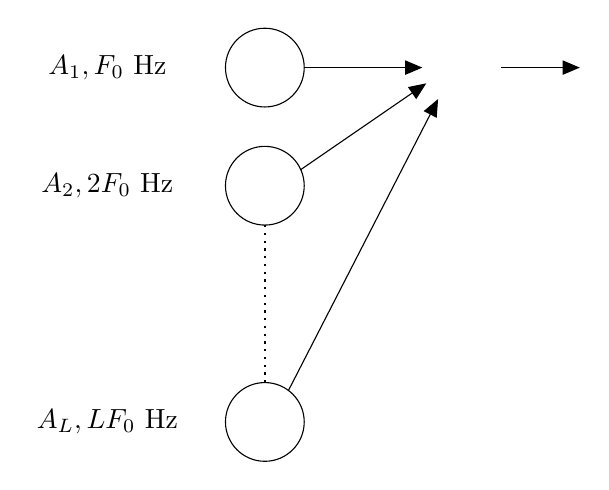
\begin{tikzpicture}[>=triangle 45,x=1.0cm,y=1.0cm]

% sine wave sources
\draw (0, 2.0) circle (0.5); \drawSine{0}{ 2.0}{0.2}{0.2}; \draw (-2.0,2.0) node {$A_1, F_0$ Hz};
\draw (0, 0.5) circle (0.5); \drawSine{0}{ 0.5}{0.2}{0.2}; \draw (-2.0,0.5) node {$A_2, 2F_0$ Hz};
\draw (0,-2.5) circle (0.5); \drawSine{0}{-2.5}{0.2}{0.2}; \draw (-2.0,-2.5) node {$A_L, LF_0$ Hz};
\draw [dotted,thick] (0,0) -- (0,-2);

\drawSummer{2.5}{2};

% connecting lines
\draw [->] (0.5,2) -- (2,2);
\draw [->] (0.45,0.7) -- (2.05,1.8);
\draw [->] (0.3,-2.1) -- (2.2,1.6);

% output speech
\draw [->] (3,2) -- (4,2);
\draw [xshift=4.2cm,yshift=2cm,color=blue] plot[smooth] file {hts2a_37_sn.txt};

\end{tikzpicture}
\end{center}
\end{figure}

The model parameters evolve over time, but can generally be considered constant for a short time window (a few 10s of ms).  For example pitch evolves over time, moving up or down as a word is articulated.

As the model parameters change over time, we need to keep updating them.  This is known as the \emph{frame rate} of the codec, which can be expressed in terms of frequency (Hz) or time (ms).  For sampling model parameters Codec 2 uses a frame rate of 10ms.  For transmission over the channel we reduce this to 20-40ms, in order to lower the bit rate.  The trade off with a lower frame rate is reduced speech quality.

The parameters of the sinusoidal model are:
\begin{enumerate}
\item The frequency of each sine wave.  As they are all harmonics of $F_0$ we can just send $F_0$ to the decoder, and it can reconstruct the frequency of each harmonic as $F_0,2F_0,3F_0,...,LF_0$.  We used 5-7 bits/frame to represent $F_0$ in Codec 2.
\item The amplitude of each sine wave, $A_1,A_2,...,A_L$.  These ``spectral amplitudes" are really important as they convey the information the ear needs to understand speech.  Most of the bits are used for spectral amplitude information.  Codec 2 uses between 18 and 50 bits/frame for spectral amplitude information.
\item Voicing information.  Speech can be approximated into voiced speech (vowels) and unvoiced speech (like consonants), or some mixture of the two.  The example in Figure \ref{fig:hts2a_time} above is voiced speech.  So we need some way to describe voicing to the decoder. This requires just a few bits/frame.
\item The phase of each sine wave.  Codec 2 discards the phases of each harmonic at the encoder and reconstruct them at the decoder using an algorithm, so no bits are required for phases.  This results in some drop in speech quality.
\end{enumerate}

\subsection{Codec 2 Encoder and Decoder}

This section explains how the Codec 2 encoder and decoder works using block diagrams.

\begin{figure}[h]
\caption{Codec 2 Encoder}
\label{fig:codec2_encoder}
\begin{center}
\begin{tikzpicture}[auto, node distance=2cm,>=triangle 45,x=1.0cm,y=1.0cm,align=center,text width=2cm]

\node [input] (rinput) {};
\node [input, right of=rinput,node distance=0.5cm] (z) {};
\node [block, right of=z,node distance=1.5cm] (pitch_est) {Pitch Estimator};
\node [block, below of=pitch_est] (fft) {FFT};
\node [block, right of=fft,node distance=3cm] (est_am) {Estimate Amplitudes};
\node [block, below of=est_am] (est_v) {Estimate Voicing};
\node [block, right of=est_am,node distance=3cm] (quant) {Decimate Quantise};
\node [output, right of=quant,node distance=2cm] (routput) {};

\draw [->] node[align=left] {Input Speech} (rinput) --  (pitch_est);
\draw [->] (z) |- (fft);
\draw [->] (pitch_est) -| (est_am);
\draw [->] (fft) -- (est_am);
\draw [->] (est_am) -- (est_v);
\draw [->] (pitch_est) -| (quant);
\draw [->] (est_am) -- (quant);
\draw [->] (est_v) -| (quant);
\draw [->] (est_v) -| (quant); 
\draw [->] (quant) -- (routput) node[right, align=left, text width=1.5cm] {Bit Stream};

\end{tikzpicture}
\end{center}
\end{figure}

The encoder is presented in Figure \ref{fig:codec2_encoder}.  Frames of input speech samples are passed to a Fast Fourier Transform (FFT), which converts the time domain samples to the frequency domain.  The same frame of input samples is used to estimate the pitch of the current frame. We then use the pitch and frequency domain speech to estimate the amplitude of each sine wave.

Yet another algorithm is used to determine if the frame is voiced or unvoiced.  This works by comparing the spectrum to what we would expect for voiced speech (e.g. lots of spectral lines).  If the energy is more random and continuous rather than discrete lines, we consider it unvoiced.

Up until this point the processing happens at a 10ms frame rate.  However in the next step we ``decimate`` the model parameters - this means we discard some of the model parameters to lower the frame rate, which helps us lower the bit rate.  Decimating to 20ms (throwing away every 2nd set of model parameters) doesn't have much effect, but beyond that the speech quality starts to degrade.  So there is a trade off between decimation rate and bit rate over the channel.

Once we have the desired frame rate, we ``quantise"" each model parameter.  This means we use a fixed number of bits to represent it, so we can send the bits over the channel.  Parameters like pitch and voicing are fairly easy, but quite a bit of DSP goes into quantising the spectral amplitudes. For the higher bit rate Codec 2 modes, we design a filter that matches the spectral amplitudes, then send a quantised version of the filter over the channel. Using the example in Figure \ref{fig:hts2a_time} - the filter would have a band pass peaks at 500 and 2300 Hz.  It's frequency response would follow the red line. The filter is time varying - we redesign it for every frame.

You'll notice the term ``estimate" being used a lot.  One of the problems with model based speech coding is the algorithms we use to extract the model parameters are not perfect.  Occasionally the algorithms get it wrong.  Look at the red crosses on the bottom plot of Figure \ref{fig:hts2a_time}.  These mark the amplitude estimate of each harmonic.  If you look carefully, you'll see that above 2000Hz, the crosses fall a little short of the exact centre of each harmonic.  This is an example of a ``fine" pitch estimator error, a little off the correct value.

Often the errors interact, for example the fine pitch error shown above will mean the amplitude estimates are a little bit off as well. Fortunately these errors tend to be temporary, and are sometimes not even noticeable to the listener - remember this codec is often used for HF/VHF radio where channel noise is part of the normal experience.
 
\begin{figure}[h]
\caption{Codec 2 Decoder}
\label{fig:codec2_decoder}
\begin{center}
\begin{tikzpicture}[auto, node distance=2cm,>=triangle 45,x=1.0cm,y=1.0cm,align=center,text width=2cm]

\node [input] (rinput) {};
\node [block, right of=rinput,node distance=2cm] (dequantise) {Dequantise Interpolate};
\node [block, right of=dequantise,node distance=3cm] (recover) {Recover Amplitudes};
\node [block, right of=recover,node distance=3cm] (synthesise) {Synthesise Speech};
\node [block, above of=synthesise] (phase) {Synthesise Phases};
\node [output, right of=synthesise,node distance=2cm] (routput) {};

\draw [->] node[align=left, text width=1.5cm] {Bit Stream} (rinput) --  (dequantise);
\draw [->] (dequantise) -- (recover);
\draw [->] (recover) -- (synthesise);
\draw [->] (recover) |- (phase);
\draw [->] (phase) -- (synthesise);
\draw [->] (synthesise) -- (routput) node[right, align=left, text width=1.5cm] {Output Speech};

\end{tikzpicture}
\end{center}
\end{figure}

Figure \ref{fig:codec2_decoder} shows the operation of the Codec 2 decoder.  We take the sequence of bits received from the channel and recover the quantised model parameters, pitch, spectral amplitudes, and voicing.  We then resample the model parameters back up to the 10ms frame rate using a technique called interpolation.  For example say we receive a $F_0=200$ Hz pitch value then 20ms later $F_0=220$ Hz.  We can use the average $F_0=210$ Hz for the middle 10ms frame.

The phases of each harmonic are generated using the other model parameters and some DSP.  It turns out that if you know the amplitude spectrum, you can determine a ``reasonable" phase spectrum using some DSP operations, which in practice is implemented with a couple of FFTs.  We also use the voicing information - for unvoiced speech we use random phases (a good way to synthesise noise-like signals) - and for voiced speech we make sure the phases are chosen so the synthesised speech transitions smoothly from one frame to the next.

Frames of speech are synthesised using an inverse FFT.  We take a blank array of FFT samples, and at intervals of $F_0$ insert samples with the amplitude and phase for each harmonic.  We then inverse FFT to create a frame of time domain samples.  These frames of synthesised speech samples are carefully aligned with the previous frame to ensure smooth frame-frame transitions, and output to the listener.

\subsection{Bit Allocation}

Table \ref{tab:bit_allocation} presents the bit allocation for two popular Codec 2 modes.  One additional parameter is the frame energy, this is the average level of the spectral amplitudes, or ``AF gain" of the speech frame.

At very low bit rates such as 700 bits/s, we use Vector Quantisation (VQ) to represent the spectral amplitudes.  We construct a table such that each row of the table has a set of spectral amplitude samples.  In Codec 2 700C the table has 512 rows.  During the quantisation process, we choose the table row that best matches the spectral amplitudes for this frame, then send the \emph{index} of the table row.  The decoder has a similar table, so can use the index to look up the output values.  If the table is 512 rows, we can use a 9 bit number to quantise the spectral amplitudes.  In Codec 2 700C, we use two tables of 512 entries each (18 bits total), the second one helps fine tune the quantisation from the first table.

Vector Quantisation can only represent what is present in the tables, so if it sees anything unusual (for example a different microphone frequency response or background noise), the quantisation can become very rough and speech quality poor.  We train the tables at design time using a database of speech samples and a training algorithm - an early form of machine learning.

Codec 2 3200 uses the method of fitting a filter to the spectral amplitudes, this approach tends to be more forgiving of small variations in the input speech spectrum, but is not as efficient in terms of bit rate.

\begin{table}[H]
\label{tab:bit_allocation}
\centering
\begin{tabular}{l c c }
\hline
Parameter & 3200 & 700C \\
\hline
Pitch $F_0$ & 7 & 5 \\
Spectral Amplitudes $\{A_m\}$ & 50 & 18 \\
Energy & 5 & 3 \\
Voicing & 2 & 1 \\
Bits/frame & 64 & 28 \\
Frame Rate & 20ms & 40ms \\
Bit rate & 3200 & 700 \\
\hline
\end{tabular}
\caption{Bit allocation of the 3200 and 700C modes}
\end{table}

\section{Detailed Design}
\label{sect:details}

\subsection{Overview}

Codec 2 is based on sinusoidal \cite{mcaulay1986speech} and Multi-Band Excitation (MBE) \cite{griffin1988multiband} vocoders that were first developed in the late 1980s.  Descendants of the MBE vocoders (IMBE, AMBE etc) have enjoyed widespread use in many applications such as VHF/UHF hand held radios and satellite communications. In the 1990s the author studied sinusoidal speech coding \cite{rowe1997techniques}, which provided the skill set and a practical, patent free baseline for starting the Codec 2 project:

Some features of Codec 2:
\begin{enumerate}
\item A range of modes supporting different bit rates, currently (Nov 2023): 3200, 2400, 1600, 1400, 1300, 1200, 700 bits/s.  These are referred to as ``Codec 2 3200", ``Codec 700C"" etc.
\item Modest CPU (a few 10s of MIPs) and memory (a few 10s of kbytes of RAM) requirements such that it can run on stm32 class microcontrollers with hardware FPU.
\item An open source reference implementation in the C language for C99/gcc compilers, and a \emph{cmake} build and test framework that runs on Linux.  Also included is a cross compiled stm32 reference implementation.
\item Ports to non-C99 compilers (e.g. MSVC, some microcontrollers, native builds on Windows) are left to third party developers - we recommend the tests also be ported and pass before considering the port successful.
\item Codec 2 has been designed for digital voice over radio applications, and retains intelligible speech at a few percent bit error rate.
\item A suite of automated tests used to verify the implementation.
\item A pitch estimator based on a 2nd order non-linearity developed by the author.
\item A single voiced/unvoiced binary voicing model.
\item A frequency domain IFFT/overlap-add synthesis model for voiced and unvoiced speech speech.
\item For the higher bit rate modes, spectral amplitudes are represented using LPCs extracted from time domain analysis and scalar LSP quantisation.
\item For Codec 2 700C, vector quantisation of resampled spectral amplitudes in the log domain.
\item Minimal interframe prediction in order to minimise error propagation and maximise robustness to channel errors.
\item A post filter that enhances the speech quality of the baseline codec, especially for low pitched (male) speakers.
\end{enumerate}

\subsection{Non-Linear Pitch Estimation}

The Non-Linear Pitch (NLP) pitch estimator was developed by the author, and is described in detail in chapter 4 of \cite{rowe1997techniques}.  There is nothing particularly unique about this pitch estimator or it's performance. Other pitch estimators could also be used, provided they have practical, real world implementations that offer comparable performance and CPU/memory requirements.  

\begin{figure}[h]
\caption{The Non-Linear Pitch (NLP) algorithm}
\label{fig:nlp}
\begin{center}
\begin{tikzpicture}[auto, node distance=2cm,>=triangle 45,x=1.0cm,y=1.0cm, align=center]

\node [input] (rinput) {};
\node [tmp, right of=rinput,node distance=0.5cm] (z) {};
\node [tmp, below of=z,node distance=1cm] (z1) {};
\node [circ, right of=z,node distance=1cm] (mult) {$\times$};
\node [block, right of=mult,node distance=2cm,text width=2cm] (notch) {DC Notch Filter};
\node [block, right of=notch,node distance=3cm,text width=2cm] (lpf) {Low Pass Filter};
\node [block, right of=lpf,node distance=2.5cm] (dec5) {$\downarrow 5$};
\node [block, below of=dec5] (dft) {DFT};
\node [block, below of=lpf] (peak) {Peak Pick};
\node [output, left of=peak,node distance=2cm] (routput) {};

\draw [->] node[align=left,text width=2cm] {Input Speech} (rinput) -- (mult);
\draw [->] (z) -- (z1) -| (mult);
\draw [->] (mult) -- (notch);
\draw [->] (notch) -- (lpf);
\draw [->] (lpf) -- (dec5);
\draw [->] (dec5) -- (dft);
\draw [->] (dft) -- (peak);
\draw [->] (peak) -- (routput) node[left, align=center] {Pitch\\Candidates};

\end{tikzpicture}
\end{center}
\end{figure}

\subsection{Sinusoidal Analysis and Synthesis}

\subsection{LPC/LSP based modes}

\subsection{Codec 2 700C}

\section{Further Work}

\begin{enumerate}
\item some examples aimed at the experimenter - e.g. using c2sim to extract and plot model parameters
\item How to use tools to single step through codec operation
\item table summarising source files with one line description
\item Add doc license (Creative Commons?)
\end{enumerate}


\bibliographystyle{plain}
\bibliography{codec2_refs}
\end{document}
